\section{Elméleti alapok}

\subsection{Mikrovezők}

A mikrovezérlők már a elterjedtek a háztartási eszközök körében is. Legfőképpen az
általánosságuk miatt, vagyis egyszerű különböző eszközöket vezérelni velük miközben 
az általánosságukból fakadóan alacsony az áruk.

Amíg régen egyedileg kellett a hardvert felállítani különböző eszközöknek az 
alapoktól kezdve, ami időigényes és költséges, mivel egy mérnök csapat meg kell 
tervezze, tesztelje és kivitelezze ami az alacsony darabszám miatt költséges egy 
darabra nézve. Ennek a hátránya ezen kívül még az, hogy nehezen módosítható és még 
hasonló eszközök eszközök közt sem cserélhetőek. Viszont maga a rendszer hatékonyabb
lehetett, mintha egy általános rendszerből lett volna kialakítva, ha a működés 
szempontjából van vizsgálva.

Manapság sokkal jobban megéri tömeggyártani egy mikroprocesszort ami általánosan 
használható rengeteg különböző eszközben, miközben a rendszerhez csupán hozzá kell 
csatolni a szenzorokat. Ehhez még nagy segítség a standardizált kommunikációs 
protokollok is a szenzorokkal, amely segítségével könnyedén összekapcsolhatóak 
a mikrovezérlővel, legtöbb esetben hardver szinten ismeri ezeket a protokollokat 
így gyorsan és hatékonyan képes kommunikálni. A leggyakrabban használt protokollok 
az $I^2C$ és SPI. Viszont manapság sok mikrovezérlőn a WiFi és Bluethoot is 
megtalálható amivel vezeték nélkül is össze lehet kötni az eszközöket, ezek az 
eszközök leginkább az IoT-Internet of Things (Dolgok Internete) alapú rendszerek
által használatosak.

Ezek a protokollok legtöbbször egyszerűek, így lehetséges szoftveresen is 
megvalósítani viszonylag egyszerűen a mikrovezérlő digitális kimeneteit használva. 
Viszont ezzel az a gond, hogy helyet foglal a memóriában, így nagy projektek esetén 
memória gondok léphetnek fel. A másik nagy gond, hogy ha időzítés érzékeny a 
protokoll akkor nehezebb betartani az időzítéseket, különösen ha nagy frekvenciájú 
jeleket kell kiküldeni. Egy ilyen példa egy VGA jel generálása, a szinkronizáló 
jelek előre meghatározott időben és csúszások nélkül kell megérkezzen, miközben 
pontos időben kell kikerüljön az adat is. Ez nehéz feladat teljes mértékben 
szoftveres megoldással megvalósítani.

Egyes mikrovezérlők ezért lehetővé tették a programozható be/kimeneteket. Ennek 
a lényege, hogy néhány kimenetet egyszer felprogramozva a processzortól függetlenül 
működik, mintha egy hardveres megvalósítás lenne, ezzel meg sokkal egyszerűbb egy 
nem alapértelmezetten támogatott protokoll megvalósítása, miközben a processzor 
nincs leterhelve ezzel a feladattal.

\subsection{Analog Digital Converter}

Az Analog Digital Converter (ADC) feladata, hogy egy analóg jelet digitális jellé
alakítson át, mivel a processzor csak digitális jeleket képes feldolgozni. Viszont 
1 bitben nem használható, mivel szinte az összes adat elveszne, ezért az ADC több 
biten tárolja el az analóg mérés eredményét. Ez legtöbbször 8-16 bit közti értékek 
közt található. A maximális érték amit az ADC eredménynek kiad az akkor történik, 
amikor az analóg jel feszültsége megegyezik az ADC referencia feszültség szintjével 
és 0 értéket ad ha a jel feszültsége 0V és a két érték között lineáris összefüggés 
van amely meredeksége 1. Erre több megoldás is létezik, viszont mindenik ugyan azt a célt éri el, 
megállapítja, hogy melyik 2 érték közé esik a feszültség szint.

Viszont ez a valóságban nem ilyen egyszerű, mivel a komponensek amik az ADC-t 
felépítik nem tökéletesek így zajok és csúszások jelenhetnek meg. Ilyen hibák 
lehetnek az offset hibák, ebben az esetben a végértékek nem felelnek meg az elvárt 
értékeknek, ilyen példa a amikor 0V-os feszültség esetén az ADC nem 0-t térít 
vissza, hanem egy nagyobb számot, míg Vref esetén egy kisebb értéket.

Az alábbi ábrán egy ilyen eset látható \ref{fig:ADC_Offset_Error} , a kék vonal az elvárt érték és a piros 
az aktuális érték, amit az ADC térít vissza a mérési tartományban. Ebben az 
esetben csupán ez a hibája az ADC-nek az átláthatóság kedvéért. 


\begin{figure}[h]
    \centering
    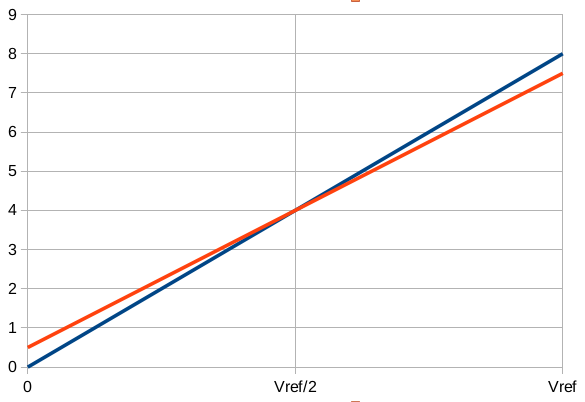
\includegraphics[scale=0.3]{figures/images/literature/ADC_Offset_Error.png}
    \caption{ADC offset hibája}
    \label{fig:ADC_Offset_Error}
\end{figure}

Másik jellegzetes hiba a nem linearitás, ennek jellemzője, hogy a mérési 
tartományon belül még az offset hibát is figyelembe véve nem azt az eredményt 
kapjuk, mint amit elvártunk amelyet nehezebb korrigálni szoftveresen, mivel amíg 
az offset hibát egyszerűen lehet korrigálni csupán a 0 és Vref feszültség szintek 
megmérésével, addig ezt a hibát sokkal nehezebb kiküszöbölni, mivel az ADC 
eredménye nem lineáris, így több ismert mérési pontot kell felvenni és a számítás 
is sokkal bonyolultabbá válik. Ezen kívül lehetnek kvantálási hibák is, amikor az 
ADC egy bizonyos értéket sosem ad eredménynek, hanem a nála egyel kisebb/nagyobb 
értéket. Ez nem okoz nagy gondot azoknál az ADC-nél ahol nagy a felbontás, viszont 
az alacsony felbontású eszközök esetén nagyobb hibát eredményez.

\section{Felhasznált technológiák}

A megvalósításhoz szükséges egy processzor, erre egy Raspberry pi pico \cite{RaspberryPico} 
mikrovezérlőt használtam. Erre a teljesítménye és alacsomy ára miatt került a választás.

%Ez egy olcső, miközben viszonylag nagy teljesítményű mikrovezérlő,
%2 hardwer szintű SPI \cite{SPIprotokol} csatornát és 3 darab 12 bites ADC-t tartalmaz.
%Erre a választás azért került, mivel még a terv kigondolása előtt már tulajdonomban volt. ,
%Hasonló mikrovezérlők vagy költségesebbek (pl. ESP32), vagy nagyon optimalizálni kellene a programot, 
%hogy ne lépje túl a hardver limitációjait (pl. Arduino).

A projekt tartalmaz egy ILI9341 \cite{ILI9341Datasheet} színes kijelzőt is, erre a nagy kijelző méret és 
nagy felbontás miatt esett a választás, hogy majd könnyedén látható legyen a mérés eredménye.

Ezen kívül használtam egy DAC8565 digital-alalóg átalakító, TS5A3357 analóg kapcsolót, és egy LP2950CZ-3.3
3.3V-os feszültség referenciát.

A pontos részleteket az a következőkben lesznek leírva.

\section{A rendszer Blokk váza}

Az alábbi árbán \ref{fig:blockDiagramm} lárható a rendszer blockDiagrammja, a fő vezérlő jelekkel.
A rendszer 2 SPI perifériával kommunikál, ezek a kijelző és a DAC, az analóg kapcsoló vezérlő jelei 
egyszerű digitális jelek, mint ahogyan a LED vezérlő jelei. A teszter socket mindhárom lába egy-egy ADC
csatornához van csatlakoztatva, ezen méri a mikrovezérlő a tesztelés során a feszültség szinteket.
A kapcsoló a RUN bemenetre van kapcsolva, ez engedélyezi a mikrovezérlő futását amíg feszültség érték 
található rajta vagy nincs bekötve. Amennyiben ez földre kerül akkor a mikrovezérlő leáll és resetelődik.

A rendszerher működéséhez szükséges egy 5V-os feszültség forrás, ez lehet egy általános USB
tápforrás, vagy lehetséges direkt 5V csatlakoztatása is. Az áramerősség alacsony, így nem közelíti
meg az 500mA-es áramerősség határt amit egy átlagos USB képes leadni. Külső akkumulátorról
is táplálható. Amennyiben egy számítógéphez, vagy egy olyan eszközhöz van csatolva ami képes 
a serial portot olvasni akkor a mérési eredményeket automatikusan elküldi azon keresztül a 
másik eszköz felé. 


\begin{figure}[h]
    \centering
    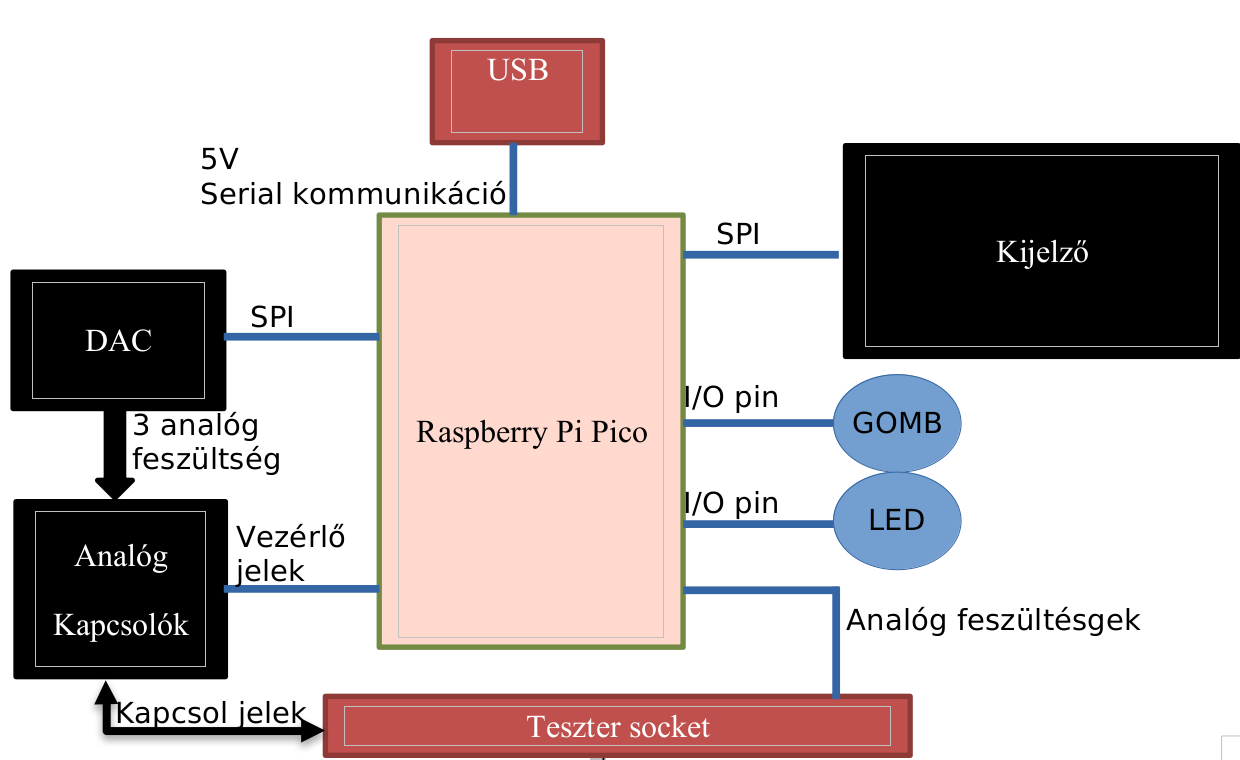
\includegraphics[scale=0.3]{figures/images/literature/blockDiagramm.png}
    \caption{A rendszer block váza}
    \label{fig:blockDiagramm}
\end{figure}







\section{Hasonló eszközök}

Egy hasonló rendszer már megvalósult \cite{similarSystem} ami egy Arduino\cite{ArduinoAtmega} 
mikroprocesszoron alapul. Ez egy egyszerűbb rendszer, ami csupán ellenállásokat használ az 
alkatrészek felismerésére és egy kijelzőt az adatok megjelenítésére. Ebből több fejlesztés is 
kialakult, több minden tesztelésére és nagyobb pontosság elérésére, miközben a rendszer 
egyszerűségét fenntartani. Ezek a rendszerek viszont nem használnak DAC-ot és ezért nem képesek 
karakterisztika diagramot készíteni. Ezen kívül nem csatlakoztatható egyszerűen számítógéphez, 
csupán újraprogramozás céljából, így minden esetben kell tartalmazzanak egy kijelzőt, ami 
növeli a költségeket. Az általános működésük hasonló, mint ebben a projektben, viszont itt 
precízen lehet változtatni a feszültséget, nem csak kapcsolni földre vagy tápfeszültségre.
Az bekötése hasonlóképpen történik: lásd \ref{fig:basicTesterConnection}

\begin{figure}[h]
    \centering
    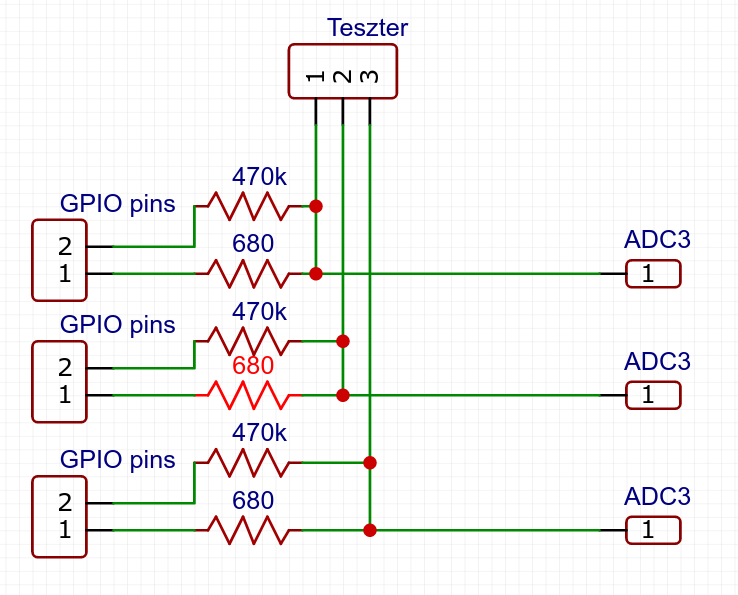
\includegraphics[scale=0.3]{figures/images/literature/OrgTesterConnection.png}
    \caption{Eredeti teszter bekötési rajza}
    \label{fig:basicTesterConnection}
\end{figure}

Mindegyik GPIO pin lehet csatolva földre, vagy tápfeszültségre, de le is lehet kapcsolva, így 
nem befolyásolja az áramkör működését. Az ADC pin meg lehet ADC üzemmódban, ilyenkor nem befolyásolja
az áramkört, viszont lehet földre, vagy tápfeszültségre is kapcsolni, ilyen esetben port ellenállás
nélkül csatolódik az áramkörre.

Viszont szintén hordozható egy 9V-os elem segítsségével és az eredmények megjelennek egy
kis LCD kijelzőn, ebből több féle verzió is létezik, van amely csak egy karakter kijelzőt
használ, van amelyik egy színes kép kirajzolására is alkalmas kijelzőt alkalmaz. 

A tesztelés néhány másodpercbe telik, nagy méretű kondenzátorok esetén telhet több időbe,
viszont ebben az esetben csak annyi idő, míg a legkissebb ellenálláson keresztül képes feltölteni
a kondenzátorot.
